
\begin{frame}
  \frametitle{Nuclear Forensics Investigations}
  \begin{adjustwidth}{-10pt}{0pt}
  \begin{figure}
    \centering
    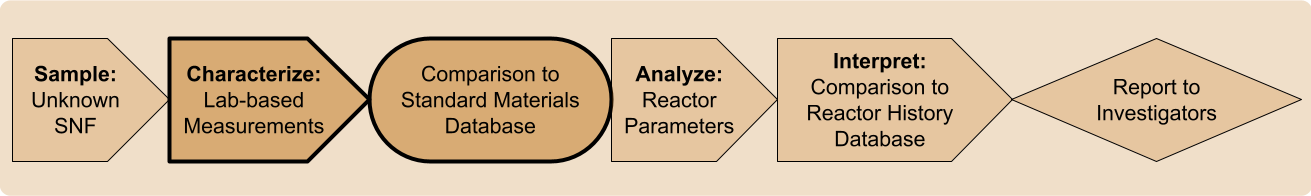
\includegraphics[width=\textwidth]{./figures/forensicsrealworld.png}
  \end{figure}
  \vspace{-3mm}
  \begin{minipage}[t]{0.5\textwidth}
    \begin{block}{Pre-detonation}
      \begin{itemize}
        \item<1-> Collection: depends on intercepted material
        \item<2-> Characterization: non-destructive and destructive
        \item<3-> Goals:
        \begin{itemize}
          \item Inverse problem: material chain of custody
          \item Safety: material handling and security
        \end{itemize}
        \item<4-> Data evaluation
      \end{itemize}
    \end{block}
  \end{minipage}%
  \hfill
  \begin{minipage}[t]{0.5\textwidth}
    \begin{block}{Post-detonation}
      \begin{itemize}
        \item<1-> Collection: debris, swipe samples
        \item<2-> Characterization: rapid analysis of isotope ratios
        \item<3-> Goals
        \begin{itemize}
          \item Inverse problem: reconstruct weapon design/yield
          \item Safety: informing disaster response
        \end{itemize}
        \item<4-> Data evaluation
      \end{itemize}
    \end{block}
  \end{minipage}
  \end{adjustwidth}
\end{frame}

\begin{frame}
  \frametitle{Attributing Spent Nuclear Fuel}
  \begin{enumerate}
    \item \textbf{Reactor Type} \\
          Classified as one of three common types of commercial power reactors:
          \begin{itemize}
            \item Pressurized water reactor (PWR)
            \item Boiling water reactor (BWR)
            \item Pressurized heavy water reactor (PHWR)
          \end{itemize}
    \item \textbf{Burnup} \\
          How much energy was produced by the fuel: megawatt-days (or 
          gigawatt-days) per metric ton of initial uranium: $\mathbf{MWd/MTU}$ 
          ($GWd/MTU$)
    \item \allbold{${}^{235}\text{U}$} \textbf{Enrichment} \\
          Percentage of ${}^{235}\text{U}$ with respect to total uranium in 
          fuel: \allbold{$\%\:{}^{235}\text{U}$}
    \item \textbf{Time Since Irradiation} \\
          How long fuel has been out of reactor core (aka cooling time): 
          $\mathbf{days}$ or $years$
  \end{enumerate}
\end{frame}


\begin{frame}
  \frametitle{Machine Learning Approach}
  \begin{adjustwidth}{-10pt}{-10pt}
  \begin{figure}
    \centering
    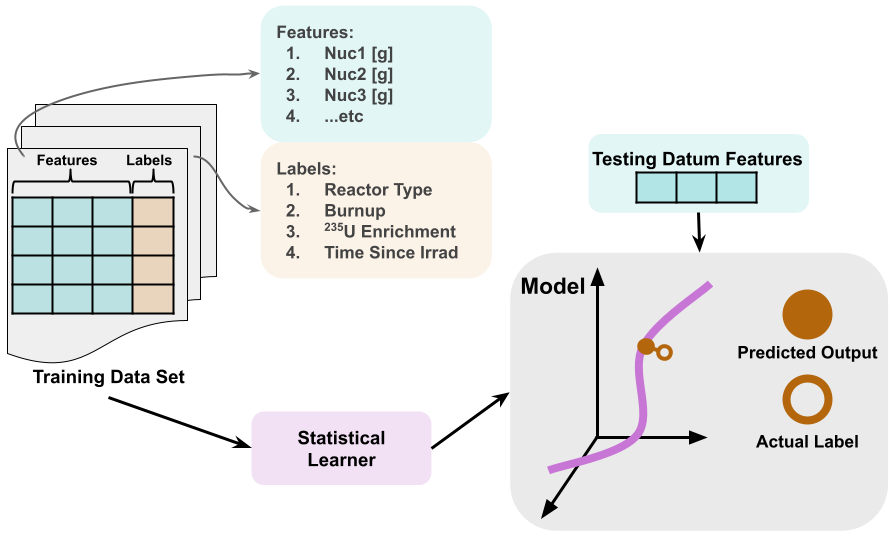
\includegraphics[width=1.05\textwidth]{./figures/pres_version_SupervisedRegression.png}
  \end{figure}
  Training and predicting using supervised regression (classification not shown)
  \end{adjustwidth}
\end{frame}

